%\section{Coupling by location shifting}
%coupling_shifting
As a 3D model the waveguide can be shifted on transverse (Fig. \ref{fig:shift_x_axis} and Fig. \ref{fig:shift_y_axis}) or longitude (Fig. \ref{fig:shift_z_axis})  directions.
\begin{figure}[!ht]
\centering
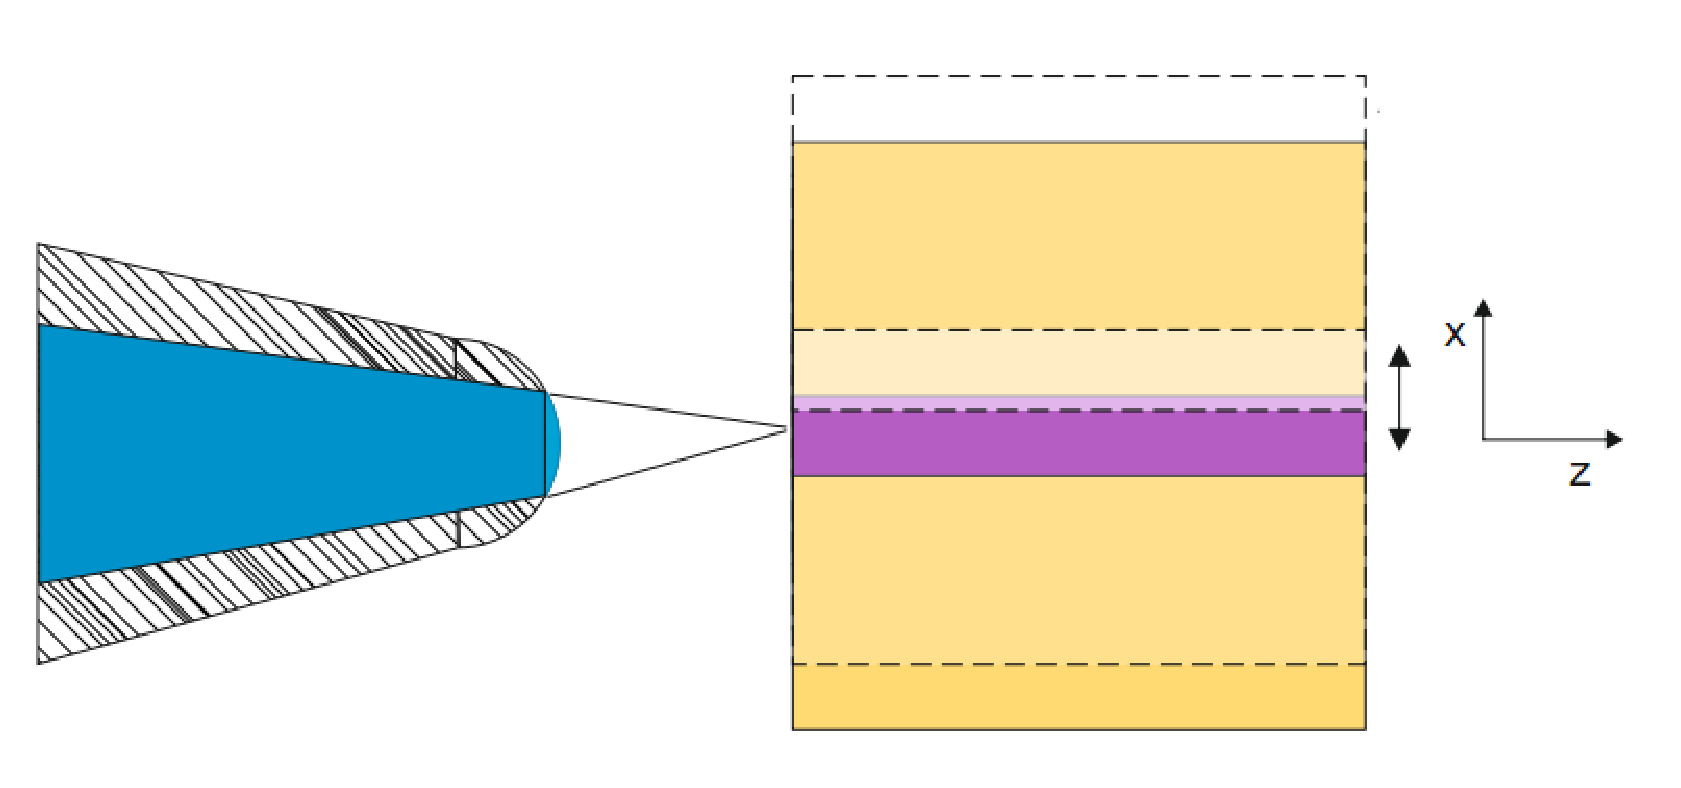
\includegraphics[width=0.6\textwidth]{bilder/shift_x_axis}
\caption{Displacing the waveguide along x-axis}
\label{fig:shift_x_axis}
\end{figure}
\begin{figure}[!ht]
\centering
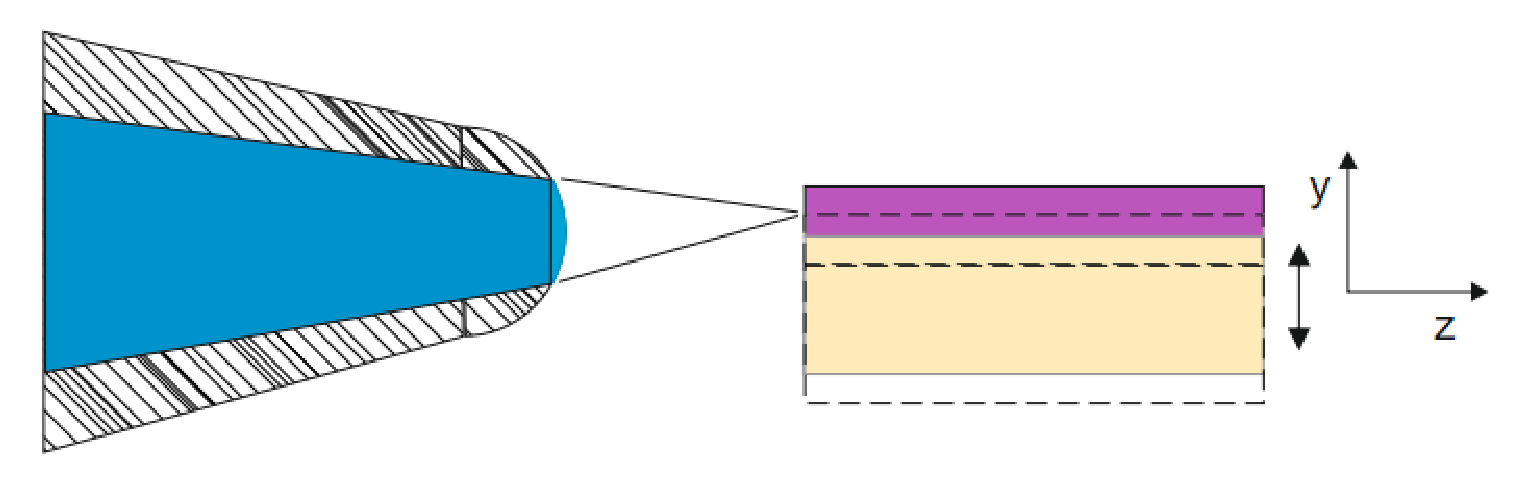
\includegraphics[width=0.6\textwidth]{bilder/shift_y_axis}
\caption{Displacing the waveguide along y-axis}
\label{fig:shift_y_axis}
\end{figure}
\begin{figure}[!ht]
\centering
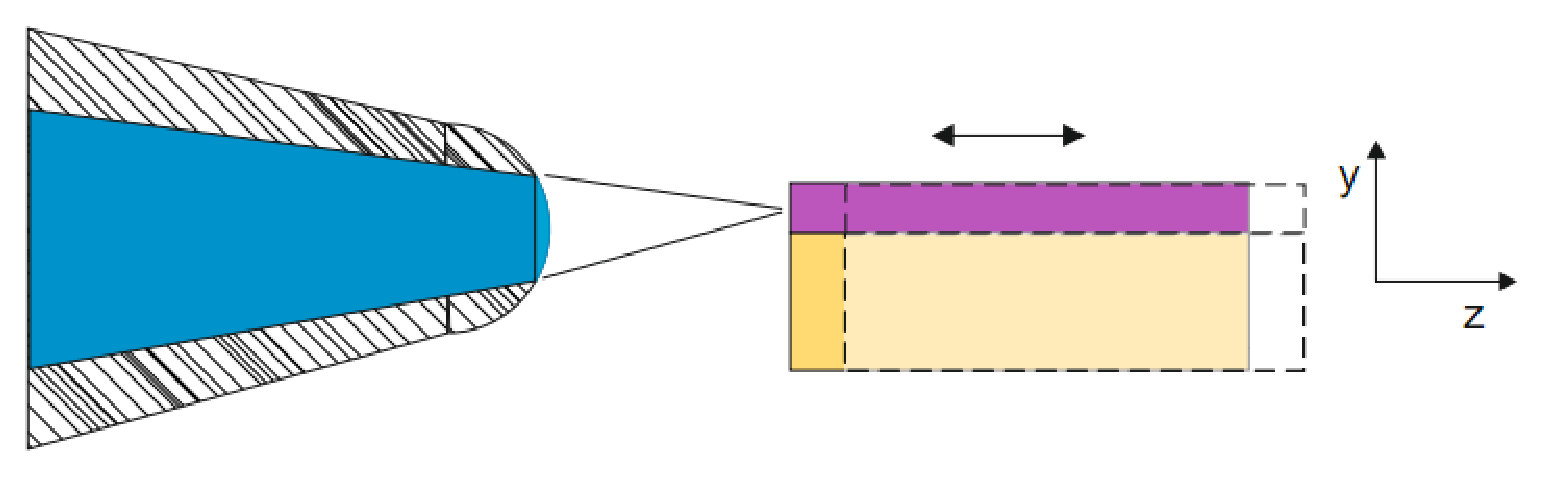
\includegraphics[width=0.6\textwidth]{bilder/shift_z_axis}
\caption{Displacing the waveguide along z-axis}
\label{fig:shift_z_axis}
\end{figure}
Shift the waveguide along X-Axis: Relocate the waveguide from $-0.4\mu$m to $0.4\mu$m and record their forward gain $S21$:
%\begin{figure}[!ht]
%\centering
%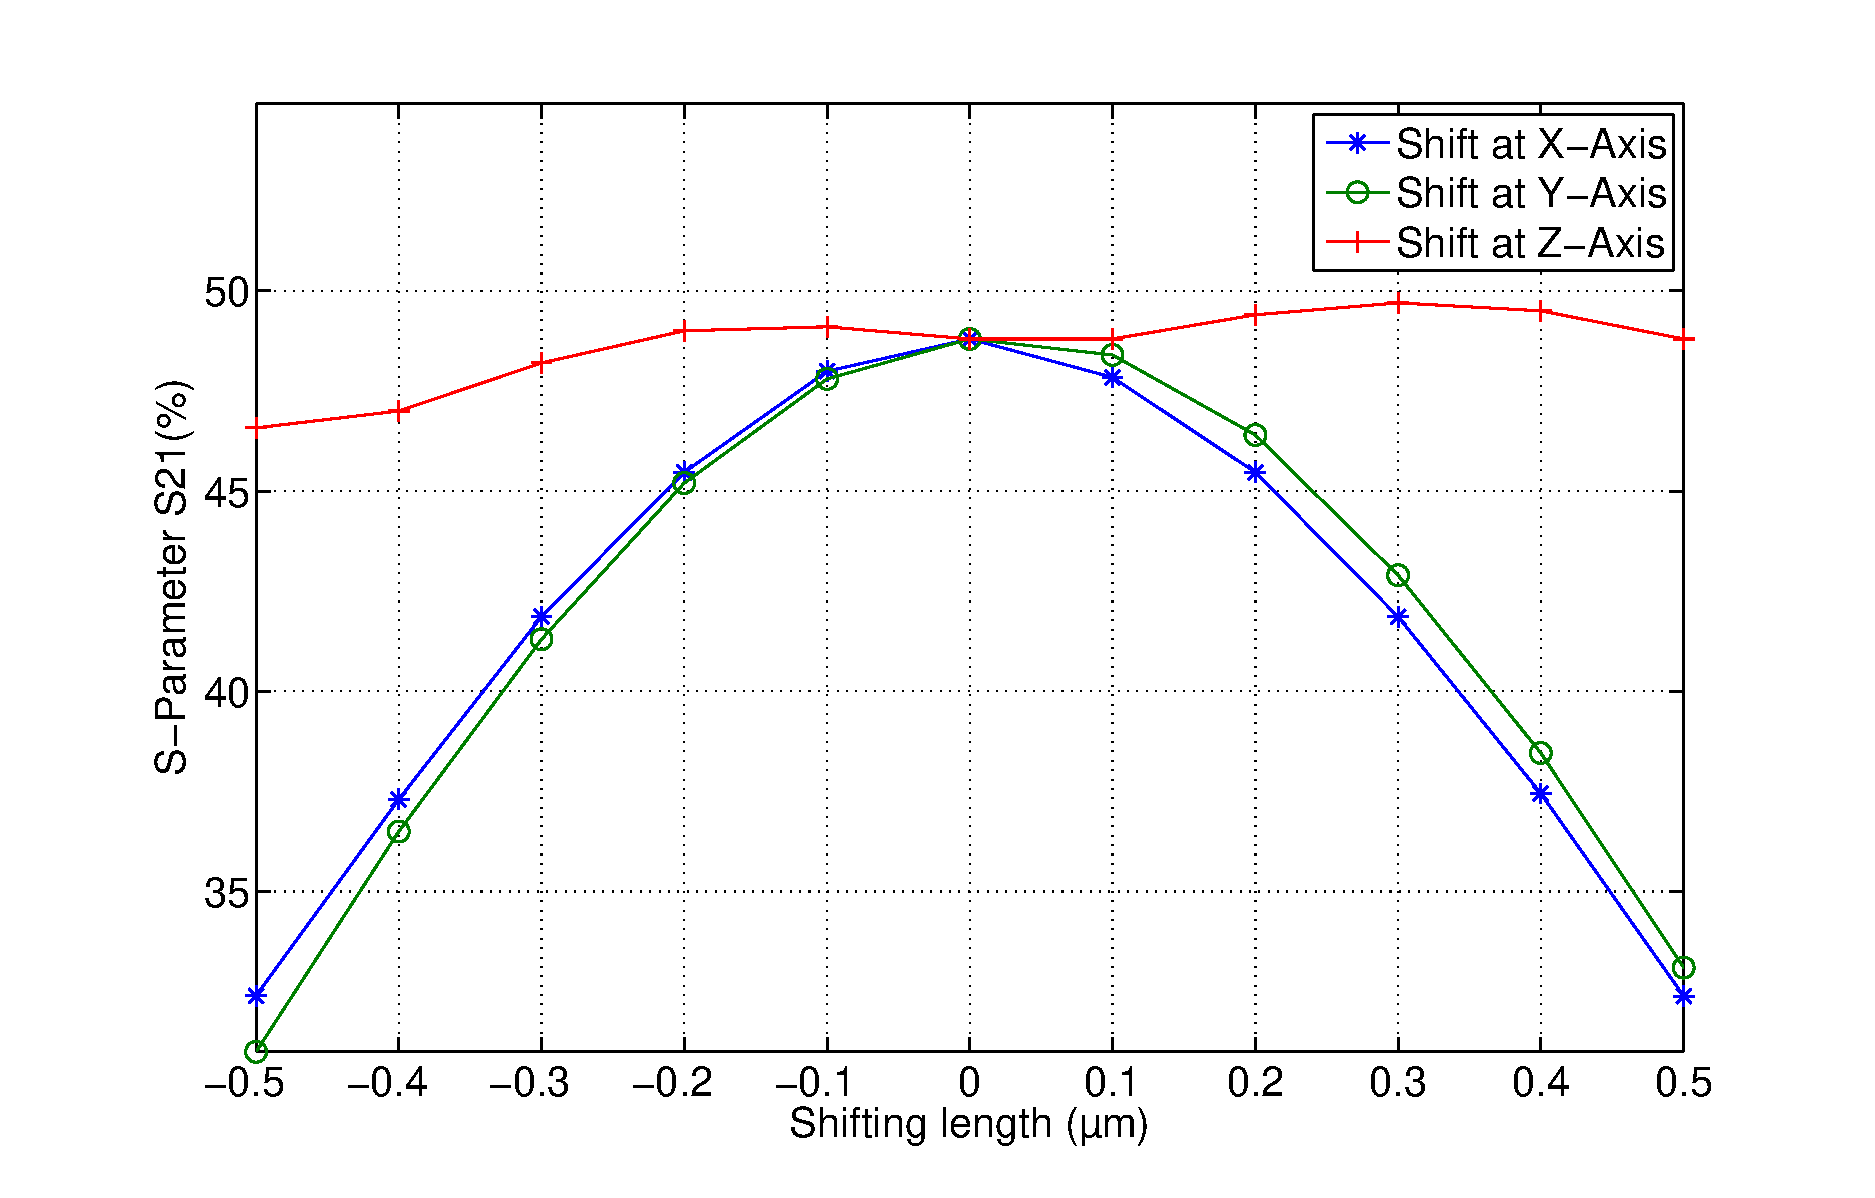
\includegraphics[width=0.6\textwidth]{bilder/shift_curve}
%\caption{Coupling efficiency due to the displacement the waveguide along x-axis}
%\label{fig:efficiency_shift_x_axis}
%\end{figure}
%
%Shift the waveguide along Y-Axis: Relocate the waveguide from $-0.4\mu$m to $0.4\mu$m and record their forward gain $S21$:
%\begin{figure}[!ht]
%\centering
%%\includegraphics[width=0.6\textwidth]{bilder/ }
%\caption{Coupling efficiency due to the displacement the waveguide along y-axis}
%\label{fig:efficiency_shift_y_axis}
%\end{figure}
%
%Shift the waveguide along Z-Axis: Relocate the waveguide from $-0.4\mu$m to $0.4\mu$m and record their forward gain $S21$: 
%\begin{figure}[!ht]
%\centering
%%\includegraphics[width=0.6\textwidth]{bilder/ }
%\caption{Coupling efficiency due to the displacement the waveguide along z-axis}
%\label{fig:efficiency_shift_z_axis}
%\end{figure}


And all detail are listed in Tab. \ref{tab:shift_result}.
\begin{table}
\caption{shifting the waveguide along X-Axis}
\begin{tabular}{cccc}
\hline
Shift|direction& X-Asis & Y-Axis & Z-Axis \\
\hline
$-0.4\mu$m &\\
$-0.3\mu$m &\\
$-0.2\mu$m&\\
$-0.1\mu$m&\\
$0\mu$m&\\
$0.1\mu$m&\\
$0.2\mu$m&\\
$0.3\mu$m&\\
$0.4\mu$m\\
\hline
\end{tabular}
\label{tab:shift_result}
\end{table}
Load all shifting data and draw their curves in Fig. \ref{fig:shift_curve}, which presents us their coupling efficiency behavior. It is obvious that the coupling efficiency falls very quickly for vertical or horizontal shifting, while it stays relative stable for longitude displacement. From this Figure we can also reveal that coupling efficiencies are symmetric due to positive and negative X-Axis shifting. While the coupling efficiencies due to negative and positive Y-Axis shifting are not symmetric. This trend can be explained by the geometric characters of the waveguide, which is same in X-Dimension and different in Y-Dimension. And the highest coupling efficiency due to shifting along Z-Axis stands not at working distance $4\mu$m but $4.3\mu$m, which agree with the estimation of minimum spot location about $4.26\mu$m at sectionXXXXX.
  
\begin{figure}[!ht]
\centering
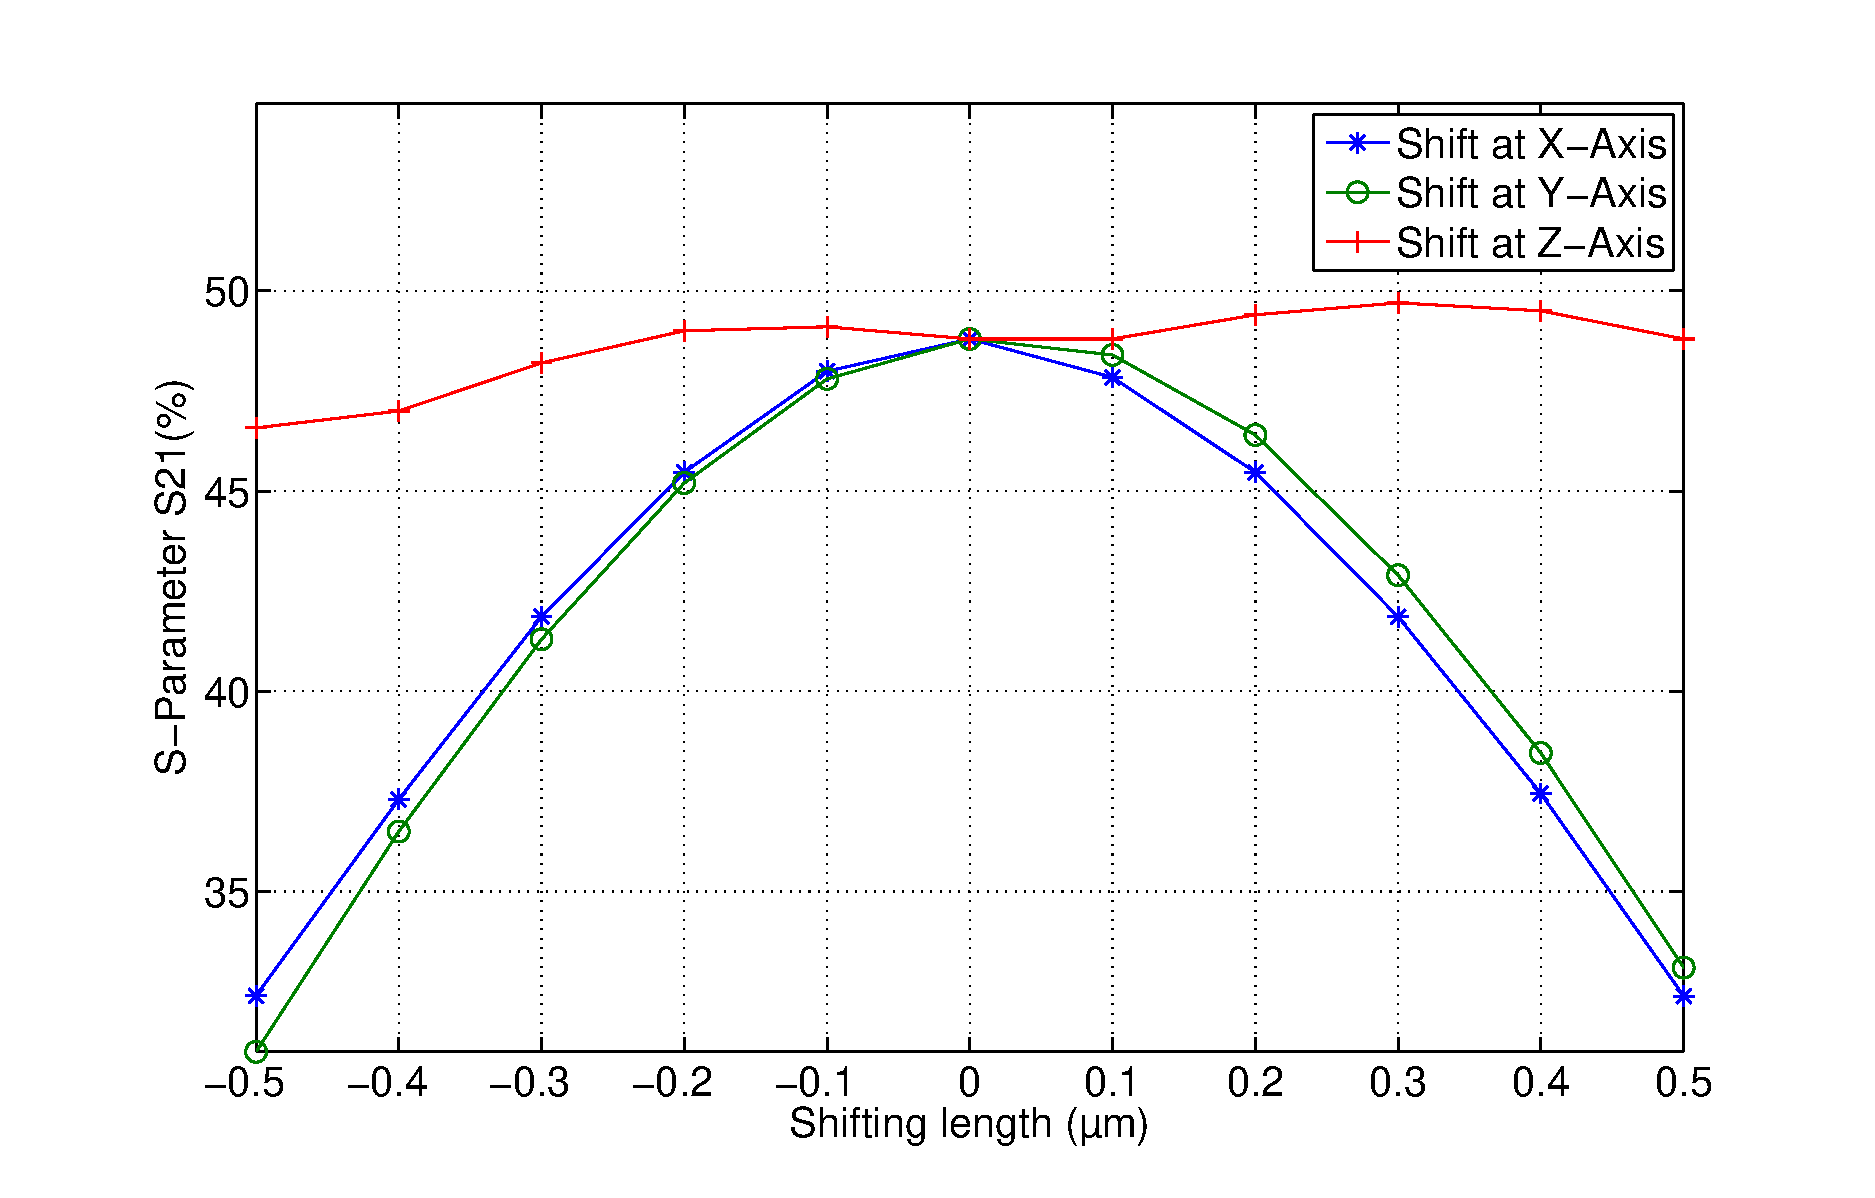
\includegraphics[width=0.6\textwidth]{bilder/shift_curve}
\caption{Coupling efficiency due to the displacement of the wavguide.}
\label{fig: shift_curve}
\end{figure}
